\documentclass[12pt,a4paper,openright,twoside]{book}
\usepackage[utf8]{inputenc}
\usepackage{disi-thesis}
\usepackage{code-lstlistings}
\usepackage{notes}
\usepackage{shortcuts}
\usepackage{acronym}

\school{\unibo}
\programme{Corso di Laurea Magistrale in Ingegneria e Scienze Informatiche}
\title{Overview, study and comparison of automation tools}
\author{Alberto Donati}
\date{\today}
\subject{Distributed Systems}
\supervisor{Prof. Giovanni Ciatto}
%\cosupervisor{Dott. CoSupervisor 1}
%\morecosupervisor{Dott. CoSupervisor 2}
\session{IV}
\academicyear{2022-2023}

% Definition of acronyms
%\acrodef{IoT}{Internet of Thing}
%\acrodef{vm}[VM]{Virtual Machine}


\mainlinespacing{1.241} % line spacing in mainmatter, comment to default (1)

\begin{document}

\frontmatter\frontispiece

\begin{abstract}
    Considering that companies have an increasing number of servers connected to the network, IT professionals increasingly find themselves with machines on which to perform the same tasks.
    Therefore, systems that could automate tasks on large numbers of machines in parallel have been created and are increasingly being used.
    This thesis aims to compare and evaluate different server automation tools, analyzing their features, advantages, and disadvantages.
    It will then go on to provide a summary overview of the reasons why professionals choose one alternative over another.
\end{abstract}

%\begin{dedication} % this is optional
%Optional. Max a few lines.
%\end{dedication}

%\begin{acknowledgements} % this is optional
%Optional. Max 1 page.
%\end{acknowledgements}

%----------------------------------------------------------------------------------------
\tableofcontents   
\listoffigures     % (optional) comment if empty
\lstlistoflistings % (optional) comment if empty
%----------------------------------------------------------------------------------------

\mainmatter

%----------------------------------------------------------------------------------------
\chapter{Introduction}
\label{chap:introduction}
%----------------------------------------------------------------------------------------

Considering the last decades, the number of servers increased, computing capacity is increasing more and more and technologies are growing.


So, now IT companies need also technologies to manage the infrastructure they have, that could simplify and organize the jobs on servers.


There are a lot of repetitive tasks when it is needed to install and configure a server, so there are now tools to simplify it a lot and also make an automation on it.


These technologies could be called "automation tools".

Considering different DevOps technologies, this document aims to study, present and compare technologies about automation.

That document will be useful for IT students, teachers and enthusiasts who wish to manage their IT environment differently.


It will be a starting point to see what is automation tools, different types of ways to automate of these technologies, see some examples and also see and overviews and comparisons.

\section{Metology}
Starting from some technologies that it is already known, it will search for technologies similar to them.


Also, sites and theses that talk about automation will be beginning to see what technologies exist.


There will be a focus on "popular" tools in these years. Searching for technologies just created will not be the scope, and also finding technologies too old might result not useful for real use.


Technologies with no costs, an open-source project, and Apache or similar license will be preferred.


There are some technologies properties of Amazon, Google and Microsoft, even if they might be described, they will not be the focus of the document.


That research also searching for tecnologies that could be useful for multipurpose scope, always related to automation.


For example, tools might not be able only to start and configure server, but it is better if it is also possible to expand with other functions.


These tools must have a solid user base. Also, It does not search for a particular language or a single way to manage machines (for example agent-agentless).


Some tools base their automation based on YAML language (Salt, Cobbler, Ansible), and others on Ruby (Chef, Puppet).

\section{Explanation of the structure}
Initially, there will be a brief description of what the automation tools are and who uses them.


Also, there will be a brief explanation about Open Source, and its importance for the projects in our use case.


For each technology, there will be a little historical view, a little study about the open source project, the trend of the language, the community and the support.


There will be a description of the tool and its components.


Also, some info on installation and examples.


Considering that automation could be easily integrated with CI/CD, it will be searching for some sort of automatic test and checks of the technology.


Considering this research and other sources, there will be a little description of pros and cons.


At the end, there will be a summary of the research done writing that document, and make tables or similar mixing different technologies.

The structure will be something like that:

\begin{itemize}
    \item Introduction
    \item State of the art (what are automation tools, who uses, open source)
    \item for each automation tool:
    \begin{itemize}
    \item History of the technology
    \item Purpose of the technology
    \item Community, maintenance and support
    \item Main technology components
    \item Installation and examples
    \item How to test the technology
    \item Pros and Cons
    \end{itemize}
    \item Conclusions (Considerations and comparisons)
\end{itemize}


\note{At the end, describe the structure of the paper}

\chapter{State of the art}

\section{What are automation tools}
We could consider in some way that for DevOps purpose all the job we need to execute is expressed in form of code\cite{learnDevOps}.


And also the configuration of server and installation of software could do that.


Automation tools are software tools that allow you to manage, monitor, and automate operations on a large number of servers. These systems can include features such as automatic provisioning, configuration management, service orchestration, performance monitoring, and troubleshooting.


An example of these systems is \textbf{Ansible}, which uses an agentless management model to connect to servers and perform automation tasks. Other examples include Puppet, Chef, and SaltStack, which offer similar features but use different approaches for server management.


These automation systems can be particularly useful in environments with a large number of servers, where manual management of each server would be inefficient and prone to errors. Through automation, organizations can improve operational efficiency, reduce errors, and free up IT staff to focus on other works.


Automation systems aim to simplify the execution of repetitive tasks.

\section{Who uses automation tools}
Automation tools could be useful from single-use who wish to simplify some task in his home running server (or cloud), to IT companies or University from a few to thusands of servers.


Some automation tools are simpler than other, for example starting from the structure of the langague used to create automations.


Some of them also require specific knowledge(Cobbler requires PXE).


There are some that could be used by beginners in IT, others that require oop languages like Ruby.

\section{When it makes sense (or doesn't make sense) to automate operations}
Some questions helps to understand when an automation tool could be a great choice:
\begin{itemize}
    \item Does It need to do that job more than once?
    \item How much time did I spend to create that automation?
    \item Create that automation will save me time or is time-consuming and not useful?
    \item What is the probability that I need to do that job another time in the future?
    \item How much is the ability to use that tool?
\end{itemize}

For example, in the case that building a very particular Linux machine with a list of packages, even if only one is needed, it could be useful because If in the future another installation of the same configuration is needed, it is possible to reinstall all the systyem in a few steps.


At the same, if I need to install a number of a few packages on hundreds of server, it will be a saving time procedure.


On the other hand, we might consider also the time spend on learn the technology, if I already know that, I could automate also very simple jobs beacuse it is used to automate all.


If it is a beginner, there are some stuff that it probability has no sense to automate beacuse the effort and time do not worth it.


When someone know a tools enough, it is possible to also expand the automation for more complex jobs.

\section{What are the main tools}
Some of the tools used by the community for automation, which try to reply to the scope indicated above are:

\begin{itemize}
    \item Ansible
    \item SaltStack
    \item Chef
    \item Puppet
\end{itemize}

Every technology has some differences considering for example language to write automation, learning curve, necessity of demons, connection with machines and so on.

\section{OpenSource and Closed Source, when OpenSource becomes Closed for some use cases}
Nowadays there are a lot of companies that acquires strategically some important business related to Open Source projects.


In the last years, for example, Ansible was acquired by RedHat in 2015, GitHub was acquired by Microsoft in 2018, SaltStack was acquired from VMware in 2020.


Even if there are some problems when a company acquires a company related to a big open-source project, it doesn't mean that the technology is worse because there are companies that make a profit on it.

Usually, big tech company that acquires others related to open source contribute to the spreading and improving the technology.


It is possible to consider one of the most important examples of that in Ubuntu.


Ubuntu is one of the most popular Linux distributions, Ubuntu has great community support and behind it is the company Canonical.


Canonical helps and contributes to Ubuntu distribution but also sells some products related like support, differences updates, infrastructures.

About automation tools, for example, Red Hat offers Ansible Automation Platform:"Red Hat Ansible Automation Platform is an end-to-end automation platform to configure systems, deploy software, and orchestrate advanced workflows. It includes resources to create, manage, and scale across the entire enterprise."\cite{ansibleAutomationPlatform}.
Automation controller it is a part of Ansible Automation Platform, and there is a sort of community-supported alternative called "AWX"\cite{ansibleAwxAAP}.
Red Hat explains that Automation controller "is produced by taking selected releases of AWX, hardening them for long-term supportability, and making them available to customers as a hosted service within Red Hat Ansible Automation Platform"\cite{ansibleFaq}.

Also Salt has open source versions and an enterprise version. The open source is free and usable via a command-line interface.
The paid enterprise edition (but the prices are not available for public), SaltStack Enterprise, that adds come features as GUI and support for Windows and MacOS.
Salt offers professional services to help customers integrate with third-party systems, also, the Salt Enterprise API has many more features than the free version.\cite{saltTechTarget}


So, when a company makes a big contribution to an open-source project there could be some negative implications ( for example regarding support or licenses), but the community nonetheless takes benefits.

\chapter{Ansible}

\section{The begin of Ansible}

Michael DeHaan define Ansible:
"Ansible is a configuration management tool, deployment tool, and ad-hoc task execution tool all in one."


The observation that formed the basis of Michael DeHaan's idea was that several online stores used separate tools for configuration, deployment, and yet another for task execution. This was because there was not one technology that could perform all these functions.


He also wanted Ansible to be as extensible as possible, that is, modules could be written in any language that could return JSON or key-value pairs.

One of the basic concepts that Micheal specified from the beginning was that configuration should be extremely simple, so without using configuration files, daemons and databases. Ansible from the beginning used a file with the machines that were to be managed written on it. Only the machines described in that file were managed, in case they were not included they would not be managed.

Quoting Micheal on his motivations for creating Ansible:


"While part of starting Ansible was to show the world there was an easier way -- to take those lessons from Red Hat, the field, and a long history of building systems management applications -- it was mostly to build the tool that (A) I actually wanted to use, and (B) was a tool that you could not use for six months, come back to, and still remember. I couldn't bring myself to be settled with the tools we had to use, it was too frustrating. As a developer myself, I wanted to write development code, I didn't want to spend 50\% of my time fighting with the automation tooling and have the automation itself be a source of frustration. I wanted to help all of these IT environments I was finding myself in, and also help myself as a consumer of those environments."

The motivation of Micheal about the project was:


"As a software developer, I myself can emphasize -- the software design/development/testing process is frequently painful, and I would rather think of infrastructure as being data-driven. Data is supposed to be simple, programs are often not. This is why I made Ansible."

\subsection{History}
In 2006 Michael DeHaan was working at Red Hat's Emerging Technologies group, a research unit under Red Hat. Emerging Tech was created specifically where people could could work on virtually anything they thought people needed.


Still those years, RedHat was very interested in configuration management. An early prototype of application virtualization management used Cobbler for provisioning the base operating system and Puppet for configuring virtual machines.


This project did not take off and Michael DeHaan attributed the cause to the fact that it was complex to write the detail under virtual applications, but Red Hat virtualization was also still in its early days.


Greg DeKoenigsberg was a Fedora community character and created a group with Michael DeHaan, Adrian Likins and Seth Vidal (author of yum). They wanted to create another very democratic open-source project in Red Hat, one that could have a wide variety of contributors and solve new problems. They thought back to busrpc. This project existed because it filled the gaps between Cobbler and Puppet. Cobbler could provide a system, and Puppet could put in configuration files, but because Puppet was too declarative you couldn't use it to do things like restart servers or do all the "ad hoc" tasks. In the past, Red Hat was exploring CIM, but there were not many good implementations of API support for Linux, so it would not be possible to build an open source project that would be able to rescout community success around CIM. The idea that was followed was to create an API-like channel for managing applications to configure systems, This idea was called Func.


Func was based on a central server reaching out to a remote node to send automation orders. It was called the central server "overlord" and each of the remote machines "minions." 


Other clones of Func were also created. Fabric and Capistrano also existed, but the team of Func wanted something more of an API and less of a script. Func was later used by Tumblr, and Steve Salesvan, who was interning at Red Hat at the time, continued to maintain it for Tumblr.


Michael therefore wanted to build a configuration management system on top of Func, tentatively called "Remote Rocket Surgery."


Cobbler, Puppet and Func formed some of the earliest DevOps-friendly automation tools, with Cobbler sometimes doing the provisioning and Func being used to launch Puppet.


After leaving RedHat and a brief term at Puppet, Micheal saw that the language often divided potential users and that the most important thing in automation tools, simplicity, should be a priority.


So Ansible began as a project in the beginning of 2012. It took off quickly due to many sysadmins and developers knowing Micheal.
Also, people from Fedora Infrastructure, replaced their Puppet automation with Ansible and so Fedora help Ansible to grow and also used as a test platform.


Like Func, it pursues a "batteries included" philosophy, allowing everyone to contribute to the main modules and forming an active community of users.


After a period when Micheal was working on automation of OpenStack with Puppet, the project started to take off on GitHub, and soon the company was founded.


Ansible increased and Micheal and others had a good-sized company supporting it and more importantly, building great products on top of it.


In 2015 Ansible was acquired from RedHat\cite{ansibleRedHat}.


Now, Ansible is currently one of the most used automation tools.

\section{Purpose of the technology}
Ansible is a technology used for automation. It allows any environment to manage the automation of commands on other machines.


The files used for the description and therefore the execution of the scripts are called Playbooks.


Ansible is based on the Python language, so it is cross-platform.


Usually, its use is recommended in a Linux environment, but some features are slightly different in a Windows environment.


Considering that most servers have a Linux kernel, the tests will focus on a Linux environment.


Ansible is ideal for managing IT environments, as it can automate tasks on a multitude of nodes simultaneously.

\subsection{Best points of Ansible}
\begin{itemize}
    \item \textbf{Simple}: As syntax, the files are described in YAML language. YAML is easy to understand by those who have minimal knowledge of programming languages and is often used for configurations. In addition, most configuration management software is characterized by an agent and a server from which to start the orchestration. In this case, Ansible's agentless management makes it easy to manage machines.
    \item \textbf{Fast}: Ansible, in addition to having a low learning curve, has a fast configuration, not having agents that must be constantly active on the host machines. Ansible connects directly to the host machines via ssh, and it is enough to have Python installed on the host machines.
    \item \textbf{Efficient}: Considering that Ansible does not have active agents, this does not consume extra resources in the hosts where the automatisms are executed. Ansible take space and resources only during the execution of the activity on the controlled node.
    \item \textbf{Secure}: Considering that the connection from the manager to controlled node is via ssh, no extra open ports are required.
\end{itemize}

\section{How the tool is shown to the community}

\subsection{Who supports and maintains the project}

\subsection{Statistics}
Ansible has 
\begin{itemize}
    \item 60.1k stars
    \item 1.9k watcher
    \item 24k fork
    \item >500 issue with >30k closed
    \item >300 pull request
    \item >5000 contributors
    \item 31.8k projects use it as dependecy
\end{itemize}

We could consider the community very active, considering also that every few days a new issue appear.

\subsection{Community way to help and improve}
If someone with to be involved in the project there is the official page that explains\cite {ansibleGithub}.

\begin{itemize}
    \item Read Community Information for all kinds of ways to contribute to and interact with the project, including mailing list information and how to submit bug reports and code to Ansible.
    \item Join a Working Group, an organized community devoted to a specific technology domain or platform.
    \item Submit a proposed code update through a pull request to the devel branch.
    \item Talk to us before making larger changes to avoid duplicate efforts. This not only helps everyone know what is going on, but it also helps save time and effort if we decide some changes are needed.
    \item For a list of email lists, IRC channels and Working Groups, see the Communication page
\end{itemize}

There is also a sort of community-based platform to share collections and roles, called Ansible Galaxy\cite{ansibleGalaxy}.



The documentation of Ansible also includes instructions to use it for its projects.

Ansible-related open-source project is AWX which "provides a web-based user interface, REST API, and task engine built on top of Ansible"\cite{ansibleAWX}.

\section{Main Ansible components}

\subsection{Inventory}
            The inventory defines the nodes (also called hosts) of the infrastructure on which Ansible performs automation.
            Even if you can pass the host names from the terminal, it is good practice to create the inventory file.
            The hosts are inserted into groups, so that you can run automations on multiple hosts at the same time.
            According to the Ansible documentation on inventory management\cite{ansibleDocInventory}, you can group the machines according to the following criteria:
            
            \begin{itemize}
                \item \textbf{What:} What purpose they were created for
                \item \textbf{Where:} Where the machines are located
                \item \textbf{When:} The stage of development they are assigned to
            \end{itemize}
            
            In addition, you can also make parent-child relationships, in which each machine inserted in a child group is also part of the parent group. All that can be done usingt the \texttt{children} attribute.
            Another function that might be useful, considering the inventories, are the variables, which can be defined for the groups (and also subgroups), through the \texttt{vars} attribute.

\subsubsection{Example Inventory Ansible}

\lstinputlisting[label={lst:exampleInventoryAnsible}]{listings/exampleInventoryAnsible.yaml}

\subsection{Modules}
Modules are small programs, which are called by tasks to perform operations on machines.


There are modules for different jobs we want to perform, some are already provided by default, and can be used from package installation to DevOps workflows.


One example is package installation via apt (ansible.builtin.apt).


There are also many modules provided by the community. If the community and default modules are not enough, there is the option of creating custom modules\cite{ansibleDocNewModules}.


Ansible modules are designed to be idempotent, which means that they will make changes to managed nodes only when necessary. This ensures that managed nodes remain in the desired state, even if the playbook is run multiple times.

\subsection{Play}
The play contains the list of tasks to be executed (at least one). The play also contains the list of hosts on which the tasks will be executed; it may contain variables and other commands.


Plays within the playbook are executed from top to bottom. Considering that playbooks are written in YAML, they are easily readable.

\subsection{Task}
The Task is the action we need to execute towards the controlled machine. The commands will be executed by calling the choosen modules with various parameters.

\subsection{Playbook}
Playbook is a collection of one or more Plays.


These are sorts of books that contain different Plays, which depending on the request, will go to be executed. Playbooks use basic programming constructs such as loops and conditionals, which allows for greater flexibility in controlling the code.


Playbooks can be reused, so you can create the best combination according to your scenario.

\subsubsection{Example Playbook Ansible}

\lstinputlisting[label={lst:examplePlaybookAnsible}]{listings/examplePlaybookAnsible.yaml}

In this example, the names of Plays are \texttt{Package installation} and \texttt{Package uninstallation}.


The execution will be targeted to the host group \texttt{campusNord}, with superuser privileges, given by the attribute-value \texttt{become : yes}.


In addition, \texttt{vars} defines two variables: \texttt{package\_name\_1} and \texttt{package\_name\_2}, which represent the names of the packages to install.


The Tasks called \texttt{Install package 1} and \texttt{Install package 2} install the packages specified by the variables \texttt{package\_name\_1} and \texttt{package\_name\_2}.


Considering that Ansible is idempotent,


in case the packages were already installed in the system, Ansible will not perform any operation and will not reinstall them either. If instead the packages were not already present in the system, Ansible, through the apt module, will install them.


In the Task \texttt{Uninstall MongoDB}, the apt module takes as input directly the value \texttt{mongodb}, and sets the state to \texttt{absent} to make sure that, if present, it is removed.

%commento
%paragraph{Roles}

%Roles: i roles (ruoli) sono dei componenti dei playbook che raggruppano operazioni legate tra di loro con uno scopo specifico. Queste vengono di solito unificate per avere più riusabilità delle stesse. Se il ruolo definito è processo standard, è facile che qualcuno lo abbia già implementato e lo si può scaricare da Ansible Galaxy!.

%differenzeeee plugin e modules
%https://docs.ansible.com/ansible/latest/dev_guide/developing_locally.html#developing-locally

\section{Characteristics}

\subsection{Platforms available (Linux, Windows, MacOS)}
Ansible is natively supported in Unix platforms like Linux distributions and MACOS.


Windows in the last years supports a Linux layer directly integrated in the machine installing WSL.

WSL (Windows Subsystem for Linux) allows the installation of a Linux distribution and the use Linux commands on Windows.


About Ansible, using Windows without WSL "is not natively supported as a control node"\cite{ansibleDocInstallIntro} and also


"The Windows Subsystem for Linux is not supported by Ansible and should not be used for production systems."\cite{ansibleWinFaq}.


Besides that, it is possible to use Windows machines as hosts and run automation scripts on those.

\subsection{Ansible project}

Ansible project (not considering others project directly related) is available at \url{https://github.com/ansible/ansible}\cite{ansibleGithub}.


This project is mainly written in Python, and its License is GNU General Public License 3.0.


The automation is written in YAML, a language invented in 2001, is a very simple language based on lists mixed with dictionaries (created with key-value pairs).

\subsection{Architecture, agent or agentless}


The architecture of Ansible is agentless, it doesn't need any type of demons or particular configuration in the host machine to be controlled.


The machine that controls others connects to nodes via ssh connections. The nodes also need (to run almost all Ansible commands) Pyhton installed.


Without that it is not needed to update and manage nodes. Having an agent allows to know better the state of the machine controlled and the condition of the network .


If a technology like Ansilbe is entirely based on connection to SSH, it means that also the security of ssh is crucial.


So, there are some ways to mitigate the risk about ssh like using like instead using password use keys, and insert password for sudo privileges\cite{ansibleSSH}

%\subsection{Structure of the project}
%\subsubsection{Deep structure of the project (how it is the open source internal project)}
%\subsection{Documentation of the project}

\subsection{Extensions of the project}
In Ansible it is possible to expand functionalities using modules and plugins.


It is possible to write them. In documentation in explained that:


Plugins are pieces of code that augment Ansible’s core functionality. Ansible uses a plugin architecture to enable a rich, flexible and expandable feature set.


Ansible ships with a number of handy plugins, and you can easily write your own."\cite{ansibleDocPlugins}.


About the creation of modules, Ansible doc explains that:


"If you need functionality that is not available in any of the thousands of Ansible modules found in collections, you can easily write your own custom module. When you write a module for local use, you can choose any programming language and follow your own rules."\cite{ansibleDocNewModules}

\section{Installation}
As indicated in the official documentation\cite{ansibleDocInstall}:

Ansible community packages are distributed in two ways:

- \textbf{ansible-core}: minimalist language and runtime package that contains a set of Ansible.Builtin.

- \textbf{ansible}: a much larger package that adds a curated selection from the Ansible Collections community to automate a wide range of devices.

The official method involves pip and then installing Ansible via pip.
\begin{lstlisting}
sudo apt install python3-pip
\end{lstlisting}

\texttt{pip} takes about 250 MegaByte of disk space.

After installing pip, install Ansible(core):

\begin{lstlisting}
python3 -m pip install --user ansible-core
\end{lstlisting}

On ubuntu.04 LTS,
Considering that Python3 is pre-installed in Ubuntu, it is possible to install Ansible via \texttt{apt}.

\begin{lstlisting}
sudo apt install ansible-core
\end{lstlisting}

The installation requires only about 80 MegaByte.

\subsection{Example}

There is a very simple way to make a fast test to see if Ansible is working, following that simple tutorial\cite{ansibleRIP}.


First, create a dir to work on it with the \texttt{mkdir} command.


After that, create a file \textbf{hosts} and add remote systems how want to manage.
\begin{lstlisting}
    192.168.1.101
    192.168.1.102
\end{lstlisting}

Considering that Ansible commands other machines with SSH connection, make sure there is a connection between the machine from where the test is done and the others.

To try the connections there is a ping module already built in Ansible, it is possible to use that also using Ansible CLI.
\begin{lstlisting}
ansible all -m ping -k
\end{lstlisting}

In case of success there will be something like that:
\begin{lstlisting}
    192.168.1.101| SUCCESS => {
        "changed": false, 
        "ping": "pong"
    }
    192.168.1.102| SUCCESS => {
        "changed": false, 
        "ping": "pong"
    }
\end{lstlisting}

\section{Tecnologies for testing Ansible}
There are different types of technologies and suites to test Ansible Playbooks in different ways.


Usually it is a good practice execute test in a dev environment. So, if something brokes, we do not need to revert  a production environment.


In our case, we need to check the Ansible Playbooks.

Considering some advice taken from \textbf{Ansible for DevOps}\cite{ansibleForDevOps}, there is three type of test:


\textbf{Unit testing}, would typically apply to individual playbooks.
Run individual playbooks in an isolated environment could be done, but it could be not too useful in that case. It is useful to check the playbook syntax

\textbf{Integration testing}, is the testing of small groupings of individual units of code, to make sure they work correctly together.
Breaking an infrastructure definition into many task-specific roles and playbooks. If the Playbook has no or limited dependencies, it is possible to test each role individually in a fresh virtual machine, before you use the role as part of a full infrastructure deployment.

\textbf{Functional testing}, when there is a complete infrastructure environment, and then run tests against it to make sure everything was successfully installed, deployed, and configured. Ansible’s own reporting is helpful in this kind of testing, and there are external tools available to test infrastructure even more deeply.

That book also show some step useful to test Ansible:

\textbf{using particular moduls}
One simple way to found error in the execution in the Playbook is print variables and output. About that, it is available a \texttt{debug} module.


Debug module is useful when verbose message on the jobs inside Ansible is needed.


If an explicit test on some variable is necessary, Ansible provides the \texttt{fail} and \texttt{assert} module.


The fail and assert modules when triggered abort the playbook run.

\textbf{using yamllint}
It is better to pay attention to YAML syntax, even if it is so simple, some common error could do to some wrong spacing.


One simple way to mitigate that problem is to install a YAML Lint Tool like \textbf{yamllint}.

\textbf{using --syntax-check}
When playbook is launched with --syntax-check, in reality, the plays are not run. Instead, Ansible loads the entire playbook statically and ensures everything can be loaded without a fatal error. If you are missing an imported task file, misspelled a module name, or are supplying a module with invalid parameters, --syntax-check will quickly identify the problem.


It requires a few seconds also for very large playbooks.

\textbf{using ansible-lint}
Linting Ansible content with ansible-lint


In addition to linting structural YAML issues with yamllint, Ansible tasks and playbooks can be linted using ansible-lint.

\textbf{Ansible Molecules}
The project Ansible Molecules helps in the development and testing of Ansible content: collections, playbooks and roles\url{https://github.com/ansible/molecule}.


Also, "Molecule provides support for testing with multiple instances, operating systems and distributions, virtualization providers, test frameworks and testing scenarios." and 


"Molecule encourages an approach that results in consistently developed roles that are well-written, easily understood and maintained."\cite{ansibleMolecule}

%\subsection{Suite for check syntax}
%\subsection{Suite for check jobs}

\section{Learning curve}
Ansible has a very fast learning curve, considering that Ansible that the automation is written in YAML files.


Also, the project was written in Python, so understanding the project is also simpler than in other languages.

%\section{Pros}

%\section{Cons}

%\section{Real project use cases}



%%%%%%%%%%%%%%%%%%%%%%%%%%%%%%%%%%%%%%%%%%%%%%%%
%SALT
%%%%%%%%%%%%%%%%%%%%%%%%%%%%%%%%%%%%%%%%%%%%%%%%
\chapter{Salt}
Salt declare itself as "the world's fastest, most intelligent and scalable automation engine"\cite{saltDocAbout}.


Salt (called also SaltStack or Salt Project) is a Python written and event driven configuration management tool, available at \url{https://saltproject.io/}.


It describes itself as "SaltStack is a revolutionary approach to infrastructure management that replaces complexity with speed. SaltStack is simple enough to get running in minutes, scalable enough to manage tens of thousands of servers, and fast enough to communicate with each system in seconds."\cite{saltDocStart}


Salt users can personalizer thier experience writing their own scripts and programs, and also use prebuilt configurations created by the users community.

\section{The begin of Salt}

\subsection{History}
Salt was started as a project ideated from Thomas S. Hatch which was not satified with other open source tecnologies available\cite{saltFloss}. He decided to use the fast ZeroMQ for connections and messages between machines.

Some steps could be seen at \url{https://red45.wordpress.com/2011/05/29/salt-configuration-management/}


For example he posted about \textbf{Salt Configuration Management} when he wrote:


"The Salt configuration management took a big leap forward late last night. The capability to define more complex states in salt from the master became a reality. Salt can now define states on the master file server, and pull those states on the minions. More work still needs to be done, and we still need to write the documentation, but this is a big step forward!".


The state of machines in Salt are written on YAML, and Salt compile these configurations in Python data structure.


Following the documentation: "The core of the Salt State system is the SLS, or SaLt State file. The SLS is a representation of the state in which a system should be in, and is set up to contain this data in a simple format."\cite{saltDocSLS}.

Also, some improves are written at when he wrote about Documentation creating a post with the title \textbf{Initial Salt Docs Site Up!}.\cite{saltPost}


Considering that Salt has support also for Windows machines, we could see a first attemps of that in December 2011 with \textbf{Windows is Being Salted!} post \cite{saltPost2}.


In that post he wrote "There is no escape from the ongoing march of Salt platform support, even Windows is now controllable via Salt! While Salt on Windows is still in its infancy, Dave Boucha has accomplished it and we have pushed the needed patches upstream. This only works on the latest git checkout of Salt and 0.9.5 will include experimental support for Windows!"\cite{saltPost2}.

During years after years, Salt grow,and in the 2020 was acquired by VMware.


About the acquisition VMware said that "it's committed to preserving SaltStack's open source community after the deal closes, with Singh noting that VMware will fully support SaltStack's work on open source projects."\cite{saltAcq}


In the blog of VMware it is possible to see the confirmation about the end of the acquisition
\url{https://blogs.vmware.com/management/2020/10/vmware-completes-saltstack-acquisition-to-bolster-software-configuration-management-and-infrastructure-automation.html}

Some months prior to the acquisition there was a big security issues related to Salt described at \url{https://news.hackreports.com/critical-saltstack-vulnerability-rce-exploit/} enough important to have two CVE related, CVE-2020-11651 and CVE-2020-11652.

\section{Purpose of the technology}
Salt use a central repository to create new servers, managed them and others. It is also possible to use it to install software on them, also on hybrid infrastructures.


Useful to deploy, configure, and manage complex IT systems, Salt has the scope to ensure that all the components of the built infrastructure are operating in a consistent desired state.


Salt is useful to simplify and eliminate manual work (and so some errors) when repetitive task is needed on cluster of servers.

\subsection{Best points of Salt}

Here are some good points about Salt:
\begin{itemize}
    \item \textbf{Flexibility:} It works on Unix and also on Windows systems, but also on different types of network devices such as switches and routers from different brand.
                                It is usually used in a mode with agents called minion, but has also a limited working mode agentless.
    \item \textbf{Speed:} It works using ZeroMQ and msgpack, so the comunication in simple, light, and fast between nodes.
    \item \textbf{Idempotent:} Every time an automation is started , it always has the same end result despite of the state of a system when the run starts.
    \item \textbf{Robust:} Considering that the system is based on agent who used ZeroMQ to communicate, agent approach with a good technology made the communication where there is a better knowledge about the state of the nodes.
    \item \textbf{Secure:} It use public keys for authentication and AES encryption for payload communication
\end{itemize}

\section{How the tool is shown to the community}

\subsection{Who supports and maintains the project}
On the official GitHub repo \url{https://github.com/saltstack/salt} about the sponsor on the Salt as a project is written:


"Salt powers VMware's VMware Aria Automation Config (previously vRealize Automation SaltStack Config / SaltStack Enterprise), and can be found under the hood of products from Juniper, Cisco, Cloudflare, Nutanix, SUSE, and Tieto, to name a few.


The original sponsor of our community, SaltStack, was acquired by VMware in 2020. The Salt Project remains an open source ecosystem that VMware supports and contributes to. VMware ensures the code integrity and quality of the Salt modules by acting as the official sponsor and manager of the Salt project. Many of the core Salt Project contributors are also VMware employees. This team carefully reviews and enhances the Salt modules to ensure speed, quality, and security."\cite{saltGitHub}


Also, there is a good community of more than 2000 contributors and also hundreds of business who use it.

\subsection{Statistics}
Salt has 
\begin{itemize}
    \item 13.7k stars
    \item >500 watcher
    \item 5.5k fork
    \item >2.4k issue with >23k closed
    \item >100 pull request
    \item >2000 contributors
    \item >600 projects use it as dependecy
\end{itemize}

We could consider the community active, expecially about finding and reporting bugs.

\subsection{Community way to help and improve}


Salt has the following way to know better and partecipate to Community:
\begin{itemize}
    \item Wiki
    \item Slack
    \item IRC on LiberaChat
    \item YouTube
    \item Twitch
    \item Reddit
\end{itemize}
On Twitter Salt declare itself community as "One of the largest, friendliest, and most active open source communities in the world"\cite{saltTwitter}.
It is possible ot contact directly the Community Manager, which is Jimmy Chunga, via Slack.
Also, there are some events about Salt:
"Every month, there are around a dozen opportunities to meet with other contributors and the Salt Core team and collaborate in real time. The best way to keep track is by subscribing to the Salt Project Community Events Calendar on the main https://saltproject.io website."\cite{saltGitHub}
Salt is very opened to contribution so they also have a email to contact \texttt{saltproject@vmware.com} for questions.

\section{Main Salt components}

\subsection{Salt Master}

Salt Master is used to communicate with other machines to execute commands of various type.
The technology for Communication used is ZeroMQ. Salt is usually used with agents(minion), but is also possible to make connections with nodes with SSH.

Salt ssh is not a substitute of standard communication of Salt, but is is a valid alternative but not fast as ZeroMQ\cite{saltSSH}.

Salt Manager use also Pillar with minions, that are "tree-like structures of data defined on the Salt Master and passed through to minions. They allow confidential, targeted data to be securely sent only to the relevant minion."\cite{saltDocPillar}

The Salt Master configuration file follow the follow parts to be corrected setted.
\begin{itemize}
    \item Primary configuration settings
    \item Large-scale tuning settings
    \item Security settings
    \item Salt-SSH Configuration
    \item Master Module Management
    \item State System settings
    \item File Server settings
    \item Pillar settings
    \item Reactor Settings
    \item Syndic settings
    \item Peer Publish settings
    \item Mine settings
    \item Logging settings
    \item Node Groups
    \item Range Cluster settings
    \item Windows Software Repo settings (also for legacy pre 2015.8 version)
    \item Returner settings
    \item Miscellaneous settings
    \item Keepalive settings
    \item NetAPI settings
    \end{itemize}

%\subsubsection{Example Salt Master}

\subsection{Salt Minion}
When the agent approach is used in Salt, minion is the agent. It receive commands from the Salt Master and communicate with him with the response of them. It has a own configuration file that can be easily setted. In that the location of the Salt Master needs to be indicated so the correct communication between them is correclty targeted.
Salt is useable also without minion in a agentless way.


The configuration file for minion has a lot of parameters that can be setted.
It is divided in differents parts:
\begin{itemize}
    \item Primary configuration settings
    \item Minion module management
    \item State Management Settings
    \item File Directory Settings
    \item Security settings
    \item Reactor Settings
    \item Thread settings
    \item Logging settings
    \item Module configuration
    \item Update settings
    \item Keepalive settings
    \item Windows Software settings
    \item Returner settings
    \item Miscellaneous settings
\end{itemize}

There is also a \textbf{salt-minion} command with different options:

\begin{itemize}
    \item \texttt{--version} (version of Salt which is running)
    \item \texttt{--versions-report} (program's dependencies and version number)
    \item \texttt{-h, --help} (help message)
    \item \texttt{-c CONFIG\_DIR, --config-dir\=CONFIG\_dir} (location of the Salt configuration directory.)
    \item \texttt{-u USER, --user\=USER} (user used to run)
    \item \texttt{-d, --daemon} (run as a daemon)
    \item \texttt{--pid-file} (PIDFILE)
\end{itemize}


%\subsubsection{Example of minion settings}

%\lstinputlisting[label={lst:exampleMinionSalt}]{listings/exampleMinionSalt.yaml}

\subsection{Reactor}
Salt's Reactor system listen for events, and than trigger actions in response to that event.

It is a simple interface to watching Salt's event bus for event tags that match a given pattern and then running one or more commands in response.
This system binds sls files to event tags on the master.


These sls files then define reactions. This means that the reactor system has two parts.


First, the reactor option needs to be set in the master configuration file.


The reactor option allows for event tags to be associated with sls reaction files.


Second, these reaction files use highdata (like the state system) to define reactions to be executed.\cite{saltDocReactor}

\subsection{Grains}
Salt has the ability to takes information about the target system.


This ability is called grains interface, because it presents salt with grains of information.


Grains are collected for the operating system, domain name, IP address, kernel, OS type, memory, and many other system properties.


The grains interface is made available to Salt modules and components so that the right salt minion commands are automatically available on the right systems.\cite{saltDocGrains}


\subsection{modules}
In Salt, both modules and execution modules are Python (or Cython) files that contain a set of functions which define the functionalities that Salt can perform.

\textbf{execution modules} are the functions called by the \texttt{salt} command, who simply run tasks on a node (minion).


\textbf{modules} (or also \texttt{state modules}) are used to get the system into a certain state/configuration, and also contain the logic to check if the system is already in the correct state/configuration.


\section{Characteristics}

\subsection{Platforms available (Linux, Windows, MacOS)}
Salt is natively supported in many Linux, MacOs and Windows systems.


Salt create a table with many OS and distribution with the compatibility with Salt.


That table and also a detailed explanations it is available at \url{https://docs.saltproject.io/salt/install-guide/en/latest/topics/salt-supported-operating-systems.html}.

\subsection{Salt project}
The project is available under the Apache 2.0 license. This license include very few restrictions about modification and distribution about the project.

\subsection{Architecture, agent or agentless}
The preferred approach that Salt uses, is the master-minion setup, the Salt master sends commands to the Salt minions to execute.
However, Salt also supports a mode where it can operate without a minion agent, so it is agentless.
Usually it better to use the agent mode, beacuse Salt is thinked and constructed in a way that make better, faster and more complete the use of minions.

%\subsection{Structure of the project}
%\subsubsection{Deep structure of the project (how it is the open source internal project)}
%\subsection{Documentation of the project}

\subsection{Extensions of the project}
Following the documentation about the creation of Salt execution module\cite{saltDocModules}.
It is possible to write Salt execution module it prefer, for the docs "A Salt execution module is a Python or Cython module placed in a directory called \_modules/ at the root of the Salt fileserver."
The module is also to a better management of module, it is possible to use module importing zipped (.zip) archive
All of the Salt execution modules are available to each other and modules can call functions available in other execution modules.

\section{Installation}

In the official documentation\cite{saltDocInstall} there is a table with different passages to correctly install Salt on the system.

Install the salt-master service on the node that will manage your other nodes, meaning it will send commands to other nodes. Then, install the salt-minion service on the nodes that will be managed by the Salt master.

Following that documentation it is possible to resume it in:

\begin{itemize}
    \item Before you start the installation, check the system requirements to ensure your platform is supported in the latest version of Salt and open the required network ports. Ensure you also have the correct permissions to install packages on the targeted nodes;
    \item Install the salt-master service on the node that will manage your other nodes, meaning it will send commands to other nodes. Then, install the salt-minion service on the nodes that will be managed by the Salt master;
    \item Configure the Salt minions to add the DNS/hostname or IP address of the Salt master they will connect to. You can add additional configurations to the master and minions as needed;
    \item Start the service on the master, then the minions;
    \item Accept the minion keys after the minion connects;
    \item Verify that the installation was successful by sending a test ping;
    \item Install third-party Python dependencies needed for specific modules.
\end{itemize}

There are also some other methods, that Salt reserve for users with a previous experience in Salt.

These can be summarized at:
\begin{itemize}
    \item Masterless
    \item Salt cloud
    \item Proxy minions
    \item Agentless
    \item Install Salt for development
\end{itemize}

\subsection{Example}
There is a well-written tutorial in the official documentation, available at \url{https://docs.saltproject.io/en/master/topics/tutorials/walkthrough.html}.
This tutorial include some passages like: installing Salt, starting Salt, finding the Salt master, setting up a salt minion, ecc.
There are also others guide like a tutorials about Salt States and Remote Execution and a stepbystep guide for MacOS.

\section{Tecnologies for testing Salt}
In the official documentations there are some test indicated, also with examples, available at 
\url{https://docs.saltproject.io/en/latest/topics/tutorials/writing_tests.html}


Salt comes with a powerful integration and unit test suite, that are two ways to test Salt with different approaches.
The test suite allows for the fully automated run of integration and/or unit tests from a single interface.
Salt's test suite is located under the \textbf{tests} directory in the root of Salt's code base and is divided into two main types described above.
The \textbf{unit} and \textbf{integration} sub-test-suites are located in the \textbf{tests} directory, which is where the majority of Salt's test cases are housed.\cite{saltDocTest}


Integration tests, the preferred way to test Salt, use Salt masters, minions, and a syndic(that is a sort of passthrough/intermediate Minion node) to test salt functionality directly and focus on testing the interaction of these components.
Salt's integration test runner includes functionality to run Salt execution modules, runners, states, shell commands, salt-ssh commands, salt-api commands, and more.
Since Salt is used to change the settings and behavior of systems, usually is convenient to run integration test in a subsystem.
Integration test could be written on purpose to modify the system where they are running, and they are called \textbf{destructive tests}\cite{saltDocTest}.


Unit test try to test a single implementation of a certain function and its logic. Unit tests should be used to test a function's exit points such as any return/raises statements.
In the part of documentation dedicated to unit tests, there are some example with different complexity: simple, complete, complex.
Unit tests are also useful in cases where writing an integration test might not be possible.
Even if the integration test suite is powerful it does not cover all functional areas of Salt's ecosystem (for example Proxy Minions).
Unit tests can still provide some testing support by testing the logic contained inside Proxy Minion functions.\cite{saltDocTest}.

%\subsection{Suite for check syntax}
%\subsection{Suite for check jobs}

\section{Learning curve}
The learining curve is not the fastes, has some configuration that is not intuitive as a completely agent-less way.
Also, considering that, even if is allowed, the connection is not passed by SSH; it is better to understand the ZeroMQ messaging technology.
having a basic understanding of how ZeroMQ works can help you better understand how SaltStack operates under the hood about the communication between nodes (master and minions).
But it need to be considered that the project is Python based, considered a simple language, and also the state files (to describe state of system components) is written in YAML, a very simple language to make configuration files.

%\section{Pros}

%\section{Cons}

%\section{Real project use cases}
%*****************************************
%* CHEF
%*****************************************
\chapter{Chef}
Chef is a tool for automation and configuration management that allows you to define and apply the desired state of a system or an infrastructure.
Chef even if it is not the simplest, is complete and with a lot of modules. The project is proud to be open-source.
Also, they create a cloud version that they are to discontinue(30th Nov 2024).
The Chef project is completely free to use, anyway, there are some limitations, considering that they also offer a premium version expecially created for companies.

\section{The begin of Chef}

\subsection{History}
The history of Chef start with  Adam Jacob, he create a technology for the company where he worked.
The company where Adam worked aims to build end-to-end server/deployment tools. Jacob showed Chef to Jesse Robbins, who saw its potential after running operations at Amazon.
In a Chef blog, in the beginning of 2009, Jesse wrote:
"I’m pleased to announce the release of Chef, a systems integration framework that brings the benefits of configuration management to your entire infrastructure.

With Chef, you can:

Manage your servers by writing code, not by running commands. 


Integrate tightly with your applications, databases, LDAP directories, and more.


Easily configure applications that require knowledge about your entire infrastructure."\cite{chefStory}

They founded a new company (Opscode) with Barry Steinglass, Nathen Haneysmith, and Joshua Timberman to turn Chef into a product.
Considering that this new tools create use a set of recipe, the project was named \textbf{Chef} at the end.

In 2013, there was a post by Bryan McLellan about the new API server written in Erlang:
"Erchef, the Chef 11 Server


The most significant new feature is that the Chef 11 Server is a complete rewrite of the core API server in Erlang, which we call Erchef.
We learned a lot from running Opscode Hosted Chef, the single largest Chef Server, as well as supporting our Opscode Private Chef customers.
Using these lessons and experience, we wrote the new server to be faster and more scalable, but still API compatible with the original Ruby based server."\cite{chefStory2}


On September 8, 2020, Progress announced the acquisition of Chef in September.\cite{chefStory3}


The company created was called as now, \textbf{Progress Chef}.



\section{Purpose of the technology}
"Chef is used by companies of all shapes and sizes, from tiny startups to the largest companies in the world, to create businesses where infrastructure moves as fast as software.", Adam Jacob, the main inventor of Chef, declare it about Chef.
Chef aims to speak from small to big business with that quote.

\subsection{Best points of Chef}

\begin{itemize}
\item{flexibility}: it works on differents Linux distros, MacOS and Windows
\item{Interoperability}: it works on clouds, on premise and also on hybrid systems.
\item{Easy repetitive}: it is possible to reuse code written by others to reproduce automation
\end{itemize}

\section{How the tool is shown to the community}
It is possible to see a starting point from the Chef community at \url{https://community.chef.io/}.

\subsection{Who supports and maintains the project}
The Chef project is divided into different modules, for that case, it takes the \textbf{Chef Server}\url{https://github.com/chef/chef-server},
the \textbf{Chef Infra}\url{https://github.com/chef/chef}, the \textbf{Chef Workstation}\url{https://github.com/chef/chef-workstation}.

There is an active community, at now the Project is also sustained by the company who own it, which is \textbf{Progress Chef}.
A lot of companies like Airbnb, Facebook, and Shopify contribute the Chef technology spreading by using it.

\subsection{Statistics}
Statistics about Chef Server and Chef Infra:


Chef Server


\begin{itemize}
    \item 283 stars
    \item >70 watcher
    \item 214 fork
    \item >150 issue with >700 closed
    \item >70 pull request
    \item >140 contributors
\end{itemize}


Chef Infra


\begin{itemize}
    \item 7.4k stars
    \item >300 watcher
    \item 2.6k fork
    \item >300 issue with >3k closed
    \item >40 pull request
    \item >650 contributors
    \item >10k projects use it as dependecy
\end{itemize}

It is possible to consider the community active, even if with not thousands of contributors, used by thousands of projects.


\subsection{Community way to help and improve}
There is a main link on the Chef site for community, at \url{https://community.chef.io/}.
There is a link created by Chef on purpose, at \url{https://github.com/chef/chef-oss-practices}.
Inside that there is a guide at \url{https://github.com/chef/chef-oss-practices/blob/main/CONTRIBUTING.md}.
Also, that is also defined the communications \url{https://github.com/chef/chef-oss-practices/blob/main/communication/README.md}.

There are four communication channels, each with its own specific purpose\cite{chefGithubOSSCom}:

\begin{itemize}
    \item \textbf{GitHub}: GitHub is the Chef Community's preferred durable medium for open and transparent development of software. All development conversation must be captured in GitHub. Any decisions made in internal Chef Slack channels, Zoom sessions, or any other communication medium must be summarized in GitHub. Please also link to the GitHub issue or pull request in chat once it is opened.
    \item \textbf{Community Slack}: Sometimes it will make sense to have a brief, non-durable conversation about the development of a project. Have these exchanges in Community Slack (either in a dev channel or via DM). Then, any development decisions, etc. arising from the Slack interaction should be documented in GitHub. Limit these conversations in Community Slack to development for a given project.
    \item \textbf{Mailing Lists}: The Chef Community mailing lists are hosted via Discourse. This is the best place to catch up on general and security-related announcements.
    \item \textbf{Office Hours}: Individual projects may host office hours on a periodic basis. This is a great way to get some face time with other Project Members. Each project should record and archive sessions to a public location; see individual project documentation for more details.
\end{itemize}

Also, there is some \texttt{interact way}, to know better the community:

\begin{itemize}
    \item Discourse at \url{https://discourse.chef.io/}
    \item Slack at \url{https://community.chef.io/slack}
    \item Chef Community Content Calendar at \url{https://calendar.google.com/calendar/u/0/embed?src=c_b1a1380a6f8d61aa926f1e3a495fca0db6f7094dc605f38bc15a1bfcf3343de6@group.calendar.google.com&ctz=America/New_York&pli=1}
\end{itemize}

Also, Chef has Twitch \url{https://www.twitch.tv/chefsoftware} and YouTube \url{https://www.youtube.com/getchefdotcom} channels.

\section{Main Chef components}

\subsection{Structure}
About the main structure, different from other similar tools, Chef has these 3 components:


\textbf{Workstation}
Chef Workstation is described as\cite{chefWorkstation}
"Chef Workstation gives you everything you need to get started with Chef, so you can automate how you audit, configure, and manage applications end environments".
The local machine where the automation code is created and pushed to the Server but also do other tasks such as execute remote scanning and configuration tasks.


\textbf{Server}
Chef Server is described as\cite{chefServer}
"Chef Infra Server is a hub for configuration data; storing cookbooks, node policies and metadata of managed nodes".
This is where all the code for making automation resides. It also contains all the information about nodes.


\textbf{Client}
Client(s), also called \textbf{Infra Client}, are strictly related to nodes. The machines where the code needs to execute.
Chef Infra Client is installed on each node that's managed with Chef Infra. Chef Infra Client configures the node locally by performing the tasks specified in the run-list.
Chef Infra Client will also pull down any required configuration data from the Chef Infra Server during a Chef Infra Client run.
Chef Infra is described as\cite{chefInfra}
"Chef Infra, a powerful automation platform that transforms infrastructure into code automating how infrastructure is configured, deployed and managed across any environment, at any scale".


It is possible to visualize that in that graphics\cite{chefFreeCodeCamp}


\begin{figure}[h]
    \centering
    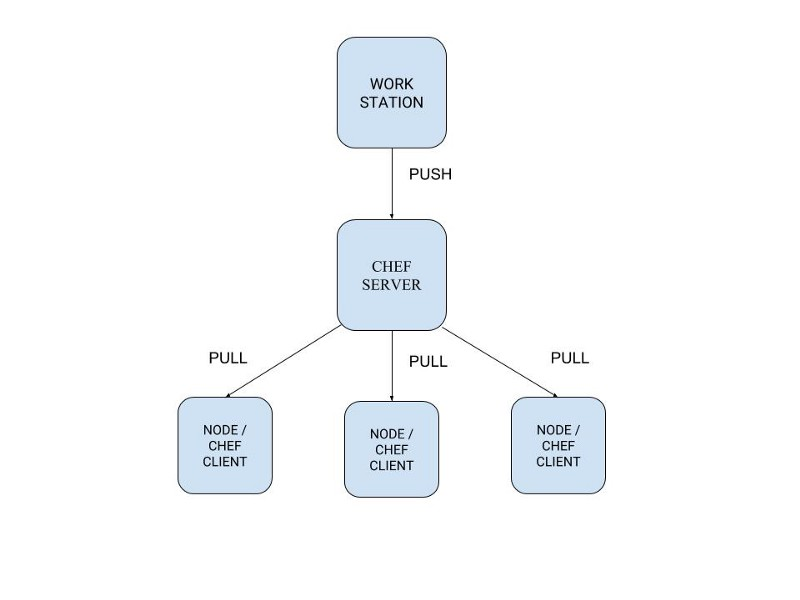
\includegraphics[width=.8\linewidth]{figures/img_Chef_structure.jpeg}
    \caption{Chef Structure}
    \label{fig:chef-structure-image}
\end{figure}

\subsection{Recipe}
Recipe is the file, written in Ruby, that contains a set of tasks to be executed step by step in the clients. It has to be in a Cookbook.

\subsection{Resource}
Resource is a piece of code that declares an element of the system and what action should be executed.
Like a sort of module in Ansible, it is possible to set the \textbf{install} and the \textbf{package} to install, for have the desired package installed.

\subsubsection{Services}
Services are used to trigger service status changes, like restarting or stopping a service.

\subsection{Cookbook}
Cookbook is a collection of recipes and other related files organized in a pre-defined way. It is created in a way to simplify the organization and sharing.

\subsection{Attributes}
Attributes are details about a specific node. Can also be defined inside recipes.
It also exists \textbf{automatic attributes} for example contain info about system.


\subsection{Example of Recipe}
An example of a recipe\cite{chefDigitalOcean}:

\lstinputlisting[label={lst:exampleRecipeChef}]{listings/exampleRecipeChef.rb}

About the recipe:

The recipe starts with an attribute definition, \texttt{node['main']['doc\_root']} where a directory is defined.


At the beginning, there are resources to \texttt{execute} a command (apt-get update), also \texttt{apt\_package} resource to install package apache2.


The service resource enables and starts the service apache2.


\texttt{directory node['main']['doc\_root'] do [...] end} defines custom attributes for that folder and create it.

A cookbook\_file resource is used to copy a local file to a remote server. This resource will copy \texttt{index.html} file and place it inside the document root created before.


In the end, the template resource applies our Apache virtual host template and notifies the service apache2 for a restart.

\section{Characteristics}

\subsection{Platforms available (Linux, Windows, MacOS)}
At \url{https://docs.chef.io/platforms/} there are written different OSs, with different sections about different Chef modules(like Infra Client, Infra Server, ecc).
The support is described as \textbf{Commercial Support} and \textbf{Community Support}.
The commercial support is described in the official Chef documentation as:
"Commercial support for platforms is part of paid maintenance contracts with Chef Software. Support contracts allow you to open tickets and receive service level agreement (SLA) assistance from our support desk. Commercially supported platforms are extensively tested as part of Chef’s development and release process. Commercial support follows the lifecycle of the underlying operating system vendor.


Commercial support is limited to the platforms listed in the “Commercial Support” tables–platforms not listed in these tables are unsupported."\cite{chefDocPlatforms}

Instead, the Community Support is considered but differently:
"Community support for platforms means that members of the Chef community have contributed to these platforms and Chef doesn’t actively work to maintain this functionality. Chef doesn’t explicitly test community supported platforms as part of the development and release process.


Many of these platforms are forks, clones, or otherwise derivative of platforms that Chef commercially supports. Continued functionality for these platforms is likely, but not guaranteed. Unsupported platforms may have missing or non-operative functionality. As always, we welcome community contributions from anyone looking to expand community support for platforms in Chef products."\cite{chefDocPlatforms}


There is also support for \textbf{Derived Platforms}, for example for a distribution that is rebuilt on an original supported distribution.

For Example, \texttt{Chef Infra Client} has Commercial Support for Amazon Linux, CentOS, Debian, FreeBSD, Ubuntu, and other Linux distros but also macOS and Windows.
It has also derived support for AlmaLinux, whose parent is CentOS but also a lot of Community Support platforms like Arch, Kali, Mint and others.

\subsection{Chef project}
The open source projects published by Chef are under Apache 2.0 license.
The main repo for Chef open source projects is \url{https://github.com/chef/}.
The Chef Server is written almost completely in Erlang and also Ruby.
Automations( inserted in Recipes ) are written in Ruby. Ruby is a free and open-source language that is not the simplest but it used for different uses, its first release was on 1995.

\subsection{Architecture, agent or agentless}
Chef works on client-server configuration with the addition of a workstation.
In Chef, there is an architecture where nodes pulls configurations (in Ruby) from the server. Chef has its own server as the source of truth that require uploaded cookbooks.
The server runs on the master machine, while the client runs as an agent on every node. Chef also has an extra component named “workstation” that stores all of the configurations that are tested then pushed to the central server.


A simplified image from the official documentation:

\begin{figure}[h]
    \centering
    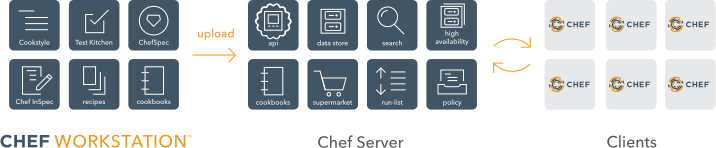
\includegraphics[width=.8\linewidth]{figures/chef_infra.png}
    \caption{Chef Infra}
    \label{fig:chef-infra-image}
\end{figure}



%Chef uses a backup server that fills in when the primary server goes down

%\subsection{Structure of the project}
%\subsubsection{Deep structure of the project (how it is the open source internal project)}
%\subsection{Documentation of the project}

\subsection{Extensions of the project}

\section{Installation}

\subsection{Example}

\section{Tecnologies for testing Chef}

%\subsection{Suite for check syntax}
%\subsection{Suite for check jobs}

\section{Learning curve}
Even if it is not the simplest, Chef has a good community with actively support the technology and other developers.
The Infra Client is written in Ruby but the server is a mix of Erlang and Ruby for most of the part.
Even if the recipes, that are written in Ruby, are not too difficult to set, Ruby is not the simplest language, in fact, in the official documentation it is possible to read about Ruby that the creator, Yukihiro Matsumoto,
"trying to make Ruby natural, not simple"\cite{rubyDoc}.

%\section{Pros}

%\section{Cons}

%\section{Real project use cases}




\chapter{Conclusion}
Scrivere la conclusione

\section{Comparison}
Esempio comparazione tecnologie

\section{Consideration}
Considerazioni finali


%\section{Some cool topic}

\chapter{Contribution}

%You may also put some code snippet (which is NOT float by default), eg: \cref{lst:random-code}.

%\lstinputlisting[float,language=Java,label={lst:random-code}]{listings/HelloWorld.java}

%\section{Fancy formulas here}

%I suggest referencing stuff as follows: \cref{fig:random-image} or \Cref{fig:random-image}

%\begin{figure}
%    \centering
%    \includegraphics[width=.8\linewidth]{figures/random-image.pdf}
%    \caption{Some random image}
%    \label{fig:random-image}
%\end{figure}

%----------------------------------------------------------------------------------------
% BIBLIOGRAPHY
%----------------------------------------------------------------------------------------

\backmatter

\nocite{*} % comment this to only show the referenced entries from the .bib file

\bibliographystyle{plainnat}
\bibliography{bibliography}

\end{document}